\chapter{Hardware and communication design}
\label{chap:comm_hardware}
%%Start af chapter:
As mentioned previously, a large portion of the project has been devoted to restructuring, and the further development of both hardware and software. Some aspects have been re-purposed to fit the previous knowledge and experience of the project managers. The goal of this chapter is to describe what physical changes have been made to the drone. It also aims to describe the general communication routine.

\section{Physical restructuring}
For finalizing the drone's basic functionality, a battery pack and wings were added to the drone. When addressing the drone, \texttt{arm 1}, \texttt{arm 2} and \texttt{arm 3} is used to denote whichever arm is in question. This applies to all chapters. 
\subsection{Wings}
The drone is retrofitted with three right-hand side wings (with respect to a normal RC plane). The wings have a length of 64 cm and a width of 20 cm at the root, which tapers into the wingtip. The chord line is the same length as the width at 20 cm (see fig. \ref{fig:wing}). The wings' camber (amount of asymmetry in relation to the chord line) was approximated to around 4\% \cite{camber, lift_coefficient}. Additionally, the wings have small winglets. Analysis of the wing's drag and lift is carried out in section \ref{chap:wing_est}. \\
Initially, other wings were chosen and ordered for the drone, but given that they were late in shipment, these wings were used instead. This resulted in use of wings with less lift, as these were smaller than the ones that were ordered. 

\begin{figure}[h!]
    \centering
    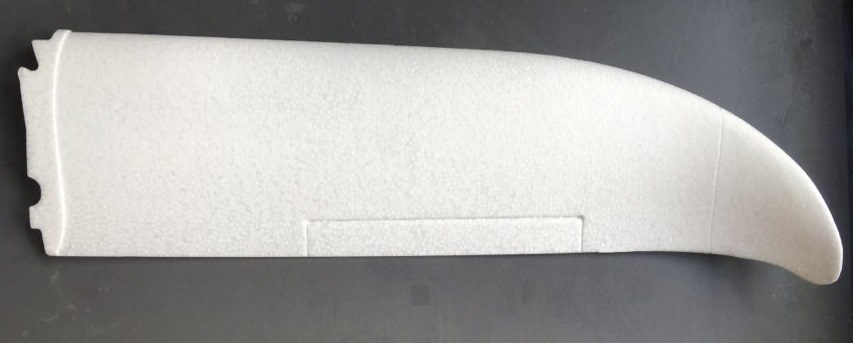
\includegraphics[width=0.9\textwidth]{figures/communication_n_hardware/wing.jpg}
    \caption{The wing type attached to each arm of the drone}
    \label{fig:wing}
\end{figure}
The wings are glued to aluminium rods and screwed into 3D printed brackets. These 3D printed brackets are attached to the servo motors of each arm, such that a rotation of the horn of the servo motor, leads to a rotation of the wing.


\subsection{Battery pack}
The battery pack consists of 3 separate Li-PO cells. Each cell has a 5000 mAh capacity at a voltage of $V_{cell} = 3.7$ V. Each cell has a discharge rate of 20C. The total weight of the battery pack containing three cells is $0.342 \,kg$. The capacity-to-weight ratio of this battery pack was deemed to be a good starting point for the drone. The cells were soldered together and placed on the bottom side of each arm to avoid interfering with the drone's center of mass \cite{battery}. The cells were wired in a series connection to reach the desired voltage of roughly 11 V.

\subsection{Additional adjustments}
In the drone's original design, each PCB was attached to the drone's frame by four elastic bands, one in each corner of the PCBs. This was done to avoid unwanted measurement errors from shaking and rattling. This design was deemed impractical, so three new modules were printed to attach the PCBs with screws to keep them static with respect to the drone's frame.\\
Moreover, each PCB was retrofitted with new voltage step-down regulators that can supply the servo motors with more power. Likewise, a faulty IMU was replaced.

\section{Data channels}
The drone's interconnected components do not require any significant communication speeds. Therefore, the I2C-protocol was deemed impractical, and further development on communication between the RPi and the Teensy via I2C was discontinued. Instead, a more convenient option of USB communication was decided upon.\\
An overview of the drone's data and power channels can be seen in fig. \ref{fig:blockdiagram}.
\begin{figure}[h!]
    \centering
    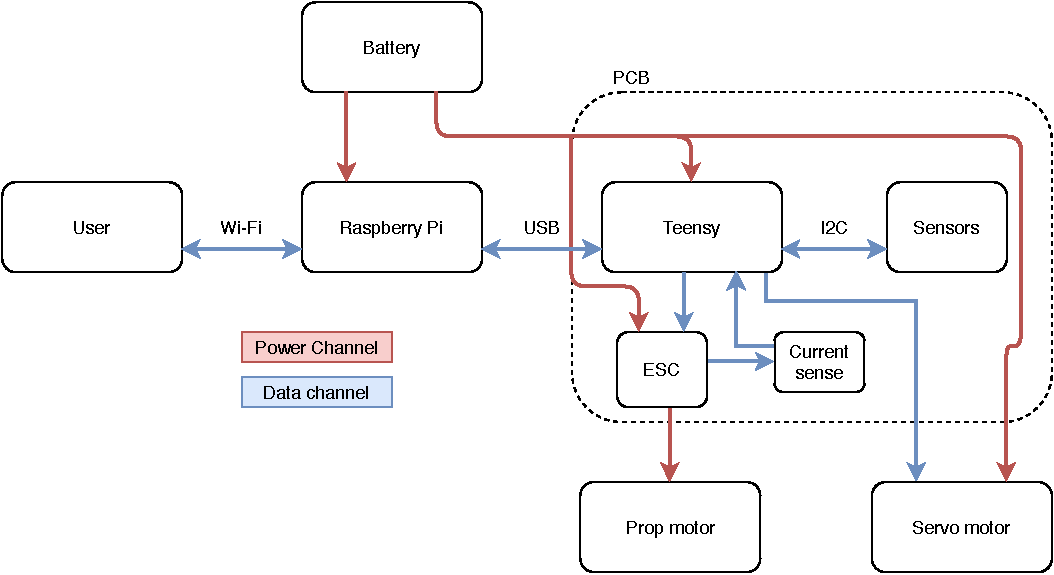
\includegraphics[width=0.75\textwidth]{figures/analysis/Propeller_Drone_Block_Diagram.pdf}
    \caption{The drone's power and data channels}
    \label{fig:blockdiagram}
\end{figure}
The previous methods for USB communication between the microcontroller and the RPi have remained. Earlier, this was only for debugging purposes, but ultimately preferred due to ease of use. The RPi sends a command, that the Teensy can interpret. The microcontroller replies via USB with the requested information. The user connects to the RPi using SSH.\\

Data between the microcontroller and the sensors was transmitted and received through the I2C-protocol. This was set up before the beginning of the project. Subsequently, this communication method has been tweaked to supply the system with reliable sensor measurements.\\ 
An interrupt pin on the IMU has been connected to the Teensy. The interrupt pin serves to signal that new data is available from the sensor. This ensures that the microcontroller receives data when available and does not need to request new data. 

\subsection{Drone routine}
The RPi and the microcontrollers are connected by USB. Information is only exchanged between the two devices when the RPi asks for it. The RPi sends a string with a distinct format specifying a command. There are two types of commands: ones that make the microcontroller return data and those that adjust values for the motors, i.e., setting a new angle for the wing tilt. The RPi is programmed in Python 3, and the microcontrollers are programmed in C++. All source code is attached to the hand-in on DTU Inside.

On the microcontroller, a buffer is filled with data from the USB connection. If the last character is an EOL sequence, a routine that reads and reacts to the information in the buffer, is invoked. For a Linux based OS, the EOL sequence typically is "\textbackslash n". 
The RPi utilizes a similar routine, also looking for a byte stream ending with an EOL sequence. The byte stream is converted to ASCII characters, and then the RPi reacts upon the data. 

For this application, the RPi has to communicate with three microcontrollers. A concurrent solution was implemented to minimize downtime when transferring data between devices. The concurrent solution was deemed superior to a sequential or parallel solution, due to the amount of IO tasks and downtime associated with waiting for data. A comparison of concurrent and parallel solutions can be seen in table \ref{tab:conccurentvsparallel}. Even though a parallel solution could potentially be faster, the before-mentioned wait time and lack of heavy computations would likely result in the same performance between the two solutions. Furthermore, the concurrent one is far easier to implement. 
\begin{table}[h]
\centering
\resizebox{\textwidth}{!}{%
\begin{tabular}{|l|l|l|}
\hline
 &
  Pros &
  Cons \\ \hline
Concurrent &
  \begin{tabular}[c]{@{}l@{}}- Ease of use\\ - Implementable on single-core systems\\ - Good for reducing down-time \\ when doing multiple IO tasks at once\end{tabular} &
  \begin{tabular}[c]{@{}l@{}}- Slower for some types of tasks\\ - Not true parallel functionality\end{tabular} \\ \hline
Parallel &
  \begin{tabular}[c]{@{}l@{}}- Generally faster when setup is done \\
  -Effective for computationally difficult\\ tasks (great for matrix multiplication,\\ 3d rendering etc.)\end{tabular} &
  \begin{tabular}[c]{@{}l@{}}- Higher complexity\\ - Need multi-core hardware\\ - Higher base resource usage\end{tabular} \\ \hline
\end{tabular}%
}
\caption{A comparison of concurrent and parallel programming}
\label{tab:conccurentvsparallel}
\end{table}

Each time the RPi needs data, it runs a function that spawns three threads. The function call takes a serial object as argument. This object defines which of the microcontrollers a given thread connects to.
The threads then communicate with the microcontrollers, and, if applicable, write data to arrays on the RPi. When finished, the threads shut down. Hereafter, new threads can be spawned with a new function call. This results in a stable sampling rate between the RPi and the microcontrollers of $f_s \approx 30 Hz$.

Typically, there can be mutual exclusion (mutex) / race condition issues when having multiple threads edit the same data, but in this application, they only edit one cell in an array with an index associated explicitly with that thread. One thread then sorts the data into the correct places. Only one thread takes care of writing data to log files. Thus, mutex issues are not a problem. 

The routine that runs on the RPi, which utilizes concurrency can be seen in fig. \ref{fig:droneroutinechart}. All communication is done using multiple threads.

\begin{figure}[h]
    \centering
    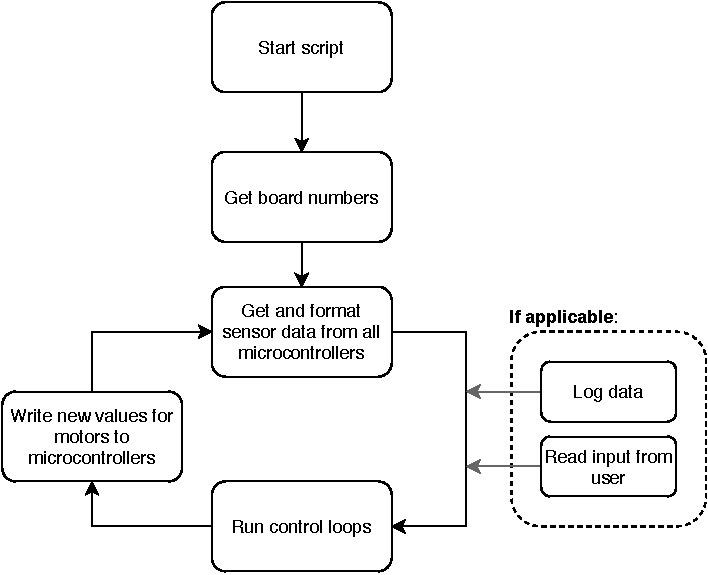
\includegraphics{figures/communication_n_hardware/droneroutine.pdf}
    \caption{A flowchart of the routine running on the RPi. After starting the script, then the board numbers are read from the microcontrollers to ensure correct indexing when writing commands to each arm. Afterwards, an infinite loop runs. User input and logging of data can be used as needed}
    \label{fig:droneroutinechart}
\end{figure}
The control loops in the routine will be examined in detail in chapter \ref{controlloopchapter}. 

Before the microcontrollers are ready to receive commands from the RPi, they perform a setup routine. Here, the microcontroller initializes all the needed IO pins, I2C and serial busses, ESC, and the IMU. The IMU performs a brief calibration of the gyroscope and accelerometer. This setup is only done once when the microcontroller boots. When this routine is done, it enters an infinite loop. 

In this loop, it receives data from the sensors, runs a filter fusion algorithm (see chapter \ref{chap:sensordataandusage}), plus checks the USB buffer and reacts upon its content, i.e., writing new PWM values to the propeller motors.
As mentioned previously, the MPU9250 is configured with an interrupt-based connection. 
This means that it sends an interrupt signal to the microcontroller, which then invokes an ISR. This routine makes the microcontroller read from the I2C connection. The interrupt signal is only sent when all registers on the MPU9250 have been filled with data. After each interrupt, the MPU9250 clears all data register and reads new data from its sensors.  

\section{Chapter summary}
The general physical construction of the drone was finished with wings, battery pack and additional components. The RPi and microcontrollers were fitted with software so they could communicate, send signals to the motors and read data from sensors. The objectives outlined in section \ref{hardwaregoals} and \ref{commgoals} have been fulfilled. Lift and drag coefficients for the wings will be estimated experimentally in section \ref{chap:wing_est}. The speed of communication between microcontrollers and RPi are commented upon in section \ref{error_measurementprecision}. All source code is attached to the hand-in on DTU Inside. 

